% Options for packages loaded elsewhere
% Options for packages loaded elsewhere
\PassOptionsToPackage{unicode}{hyperref}
\PassOptionsToPackage{hyphens}{url}
\PassOptionsToPackage{dvipsnames,svgnames,x11names}{xcolor}
%
\documentclass[
  letterpaper,
  DIV=11,
  numbers=noendperiod]{scrartcl}
\usepackage{xcolor}
\usepackage{amsmath,amssymb}
\setcounter{secnumdepth}{-\maxdimen} % remove section numbering
\usepackage{iftex}
\ifPDFTeX
  \usepackage[T1]{fontenc}
  \usepackage[utf8]{inputenc}
  \usepackage{textcomp} % provide euro and other symbols
\else % if luatex or xetex
  \usepackage{unicode-math} % this also loads fontspec
  \defaultfontfeatures{Scale=MatchLowercase}
  \defaultfontfeatures[\rmfamily]{Ligatures=TeX,Scale=1}
\fi
\usepackage{lmodern}
\ifPDFTeX\else
  % xetex/luatex font selection
\fi
% Use upquote if available, for straight quotes in verbatim environments
\IfFileExists{upquote.sty}{\usepackage{upquote}}{}
\IfFileExists{microtype.sty}{% use microtype if available
  \usepackage[]{microtype}
  \UseMicrotypeSet[protrusion]{basicmath} % disable protrusion for tt fonts
}{}
\makeatletter
\@ifundefined{KOMAClassName}{% if non-KOMA class
  \IfFileExists{parskip.sty}{%
    \usepackage{parskip}
  }{% else
    \setlength{\parindent}{0pt}
    \setlength{\parskip}{6pt plus 2pt minus 1pt}}
}{% if KOMA class
  \KOMAoptions{parskip=half}}
\makeatother
% Make \paragraph and \subparagraph free-standing
\makeatletter
\ifx\paragraph\undefined\else
  \let\oldparagraph\paragraph
  \renewcommand{\paragraph}{
    \@ifstar
      \xxxParagraphStar
      \xxxParagraphNoStar
  }
  \newcommand{\xxxParagraphStar}[1]{\oldparagraph*{#1}\mbox{}}
  \newcommand{\xxxParagraphNoStar}[1]{\oldparagraph{#1}\mbox{}}
\fi
\ifx\subparagraph\undefined\else
  \let\oldsubparagraph\subparagraph
  \renewcommand{\subparagraph}{
    \@ifstar
      \xxxSubParagraphStar
      \xxxSubParagraphNoStar
  }
  \newcommand{\xxxSubParagraphStar}[1]{\oldsubparagraph*{#1}\mbox{}}
  \newcommand{\xxxSubParagraphNoStar}[1]{\oldsubparagraph{#1}\mbox{}}
\fi
\makeatother


\usepackage{longtable,booktabs,array}
\newcounter{none} % for unnumbered tables
\usepackage{calc} % for calculating minipage widths
% Correct order of tables after \paragraph or \subparagraph
\usepackage{etoolbox}
\makeatletter
\patchcmd\longtable{\par}{\if@noskipsec\mbox{}\fi\par}{}{}
\makeatother
% Allow footnotes in longtable head/foot
\IfFileExists{footnotehyper.sty}{\usepackage{footnotehyper}}{\usepackage{footnote}}
\makesavenoteenv{longtable}
\usepackage{graphicx}
\makeatletter
\newsavebox\pandoc@box
\newcommand*\pandocbounded[1]{% scales image to fit in text height/width
  \sbox\pandoc@box{#1}%
  \Gscale@div\@tempa{\textheight}{\dimexpr\ht\pandoc@box+\dp\pandoc@box\relax}%
  \Gscale@div\@tempb{\linewidth}{\wd\pandoc@box}%
  \ifdim\@tempb\p@<\@tempa\p@\let\@tempa\@tempb\fi% select the smaller of both
  \ifdim\@tempa\p@<\p@\scalebox{\@tempa}{\usebox\pandoc@box}%
  \else\usebox{\pandoc@box}%
  \fi%
}
% Set default figure placement to htbp
\def\fps@figure{htbp}
\makeatother





\setlength{\emergencystretch}{3em} % prevent overfull lines

\providecommand{\tightlist}{%
  \setlength{\itemsep}{0pt}\setlength{\parskip}{0pt}}



 


\usepackage{float}
\usepackage{tabularray}
\usepackage[normalem]{ulem}
\usepackage{graphicx}
\usepackage{rotating}
\UseTblrLibrary{siunitx}
\NewTableCommand{\tinytableDefineColor}[3]{\definecolor{#1}{#2}{#3}}
\newcommand{\tinytableTabularrayUnderline}[1]{\underline{#1}}
\newcommand{\tinytableTabularrayStrikeout}[1]{\sout{#1}}
\KOMAoption{captions}{tableheading}
\makeatletter
\@ifpackageloaded{caption}{}{\usepackage{caption}}
\AtBeginDocument{%
\ifdefined\contentsname
  \renewcommand*\contentsname{Table of contents}
\else
  \newcommand\contentsname{Table of contents}
\fi
\ifdefined\listfigurename
  \renewcommand*\listfigurename{List of Figures}
\else
  \newcommand\listfigurename{List of Figures}
\fi
\ifdefined\listtablename
  \renewcommand*\listtablename{List of Tables}
\else
  \newcommand\listtablename{List of Tables}
\fi
\ifdefined\figurename
  \renewcommand*\figurename{Figure}
\else
  \newcommand\figurename{Figure}
\fi
\ifdefined\tablename
  \renewcommand*\tablename{Table}
\else
  \newcommand\tablename{Table}
\fi
}
\@ifpackageloaded{float}{}{\usepackage{float}}
\floatstyle{ruled}
\@ifundefined{c@chapter}{\newfloat{codelisting}{h}{lop}}{\newfloat{codelisting}{h}{lop}[chapter]}
\floatname{codelisting}{Listing}
\newcommand*\listoflistings{\listof{codelisting}{List of Listings}}
\makeatother
\makeatletter
\makeatother
\makeatletter
\@ifpackageloaded{caption}{}{\usepackage{caption}}
\@ifpackageloaded{subcaption}{}{\usepackage{subcaption}}
\makeatother
\usepackage{bookmark}
\IfFileExists{xurl.sty}{\usepackage{xurl}}{} % add URL line breaks if available
\urlstyle{same}
\hypersetup{
  pdftitle={Cultural Matching Analysis},
  pdfauthor={Omar Lizardo et al.},
  colorlinks=true,
  linkcolor={blue},
  filecolor={Maroon},
  citecolor={Blue},
  urlcolor={Blue},
  pdfcreator={LaTeX via pandoc}}


\title{Cultural Matching Analysis}
\author{Omar Lizardo et al.}
\date{2026-07-16}
\begin{document}
\maketitle

\renewcommand*\contentsname{Table of contents}
{
\setcounter{tocdepth}{3}
\tableofcontents
}

\subsection{Overview}\label{overview}

This analysis file examines the role of cultural matching and network
opacity in predicting the persistence of social ties over time. We pool
data across adjacent waves from the NetSense study to construct a
person-period dataset, restricting the sample to non-kin, on-campus
student ties. We estimate the probability of tie persistence as a
function of cultural matching (closed-form domains and open-ended
activities) and network opacity (the number of ``Don't Know'' responses
regarding an alter's preferences) using mixed-effects logistic
regression (\texttt{lme4::glmer}).

\subsection{Main Effects Models}\label{main-effects-models}

The following models assess the main effects of closed-form cultural
matching, open-ended cultural matching, and network opacity on the odds
of tie persistence. Model 1 shows that closed-form matches independently
predict persistence. Model 2 introduces open-ended matches,
demonstrating the value of incorporating both open and closed-form
items. Model 3 incorporates network opacity (the number of ``Don't
know'' responses regarding an alter's preferences). The main effects
model reveals that a lack of shared cultural knowledge signals a weaker
tie.

\subsubsection{Marginal Effects}\label{marginal-effects}

\textbf{Figure Figure~\ref{fig-combined}} visualizes the marginal effect
(calculated as the change from the minimum to the maximum value) of
closed-form matches, open-ended matches, and network opacity on the
predicted probability of tie persistence.

\begin{figure}

\centering{

\pandocbounded{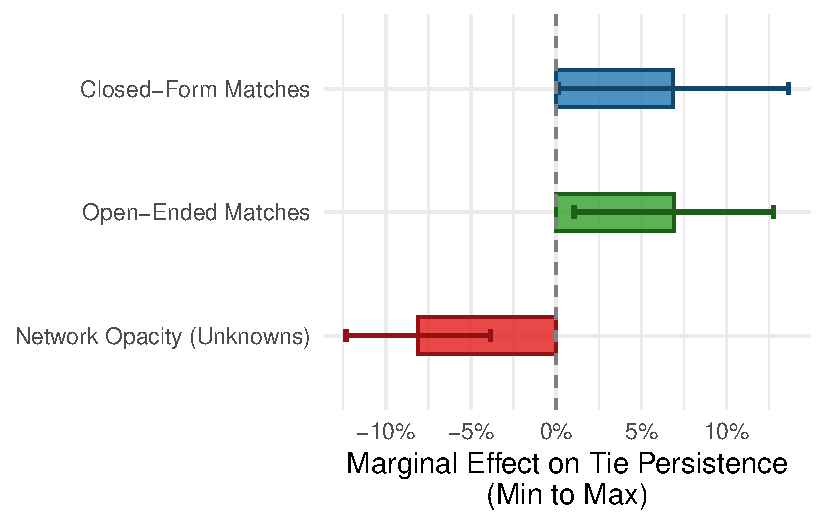
\includegraphics[keepaspectratio]{analysis_files/figure-pdf/fig-combined-1.pdf}}

}

\caption{\label{fig-combined}Marginal Effects of Cultural Matches and
Network Opacity (Min to Max)}

\end{figure}%

\subsection{Subjective Closeness
Interactions}\label{subjective-closeness-interactions}

To test whether the protective effects of cultural matching or the
detrimental effects of network opacity depend on the strength of the
tie, we estimated auxiliary interaction models between subjective
closeness and each of the three cultural variables. While interaction
terms in logistic regression models can be difficult to interpret
directly from coefficients due to the non-linear link function,
computing predicted probabilities across the range of the variables
provides a clearer picture of the underlying dynamics.

\textbf{Figure Figure~\ref{fig-closeness-interactions}} plots the
marginal effects of the three cultural variables across the three levels
of subjective closeness.

\begin{figure}

\centering{

\pandocbounded{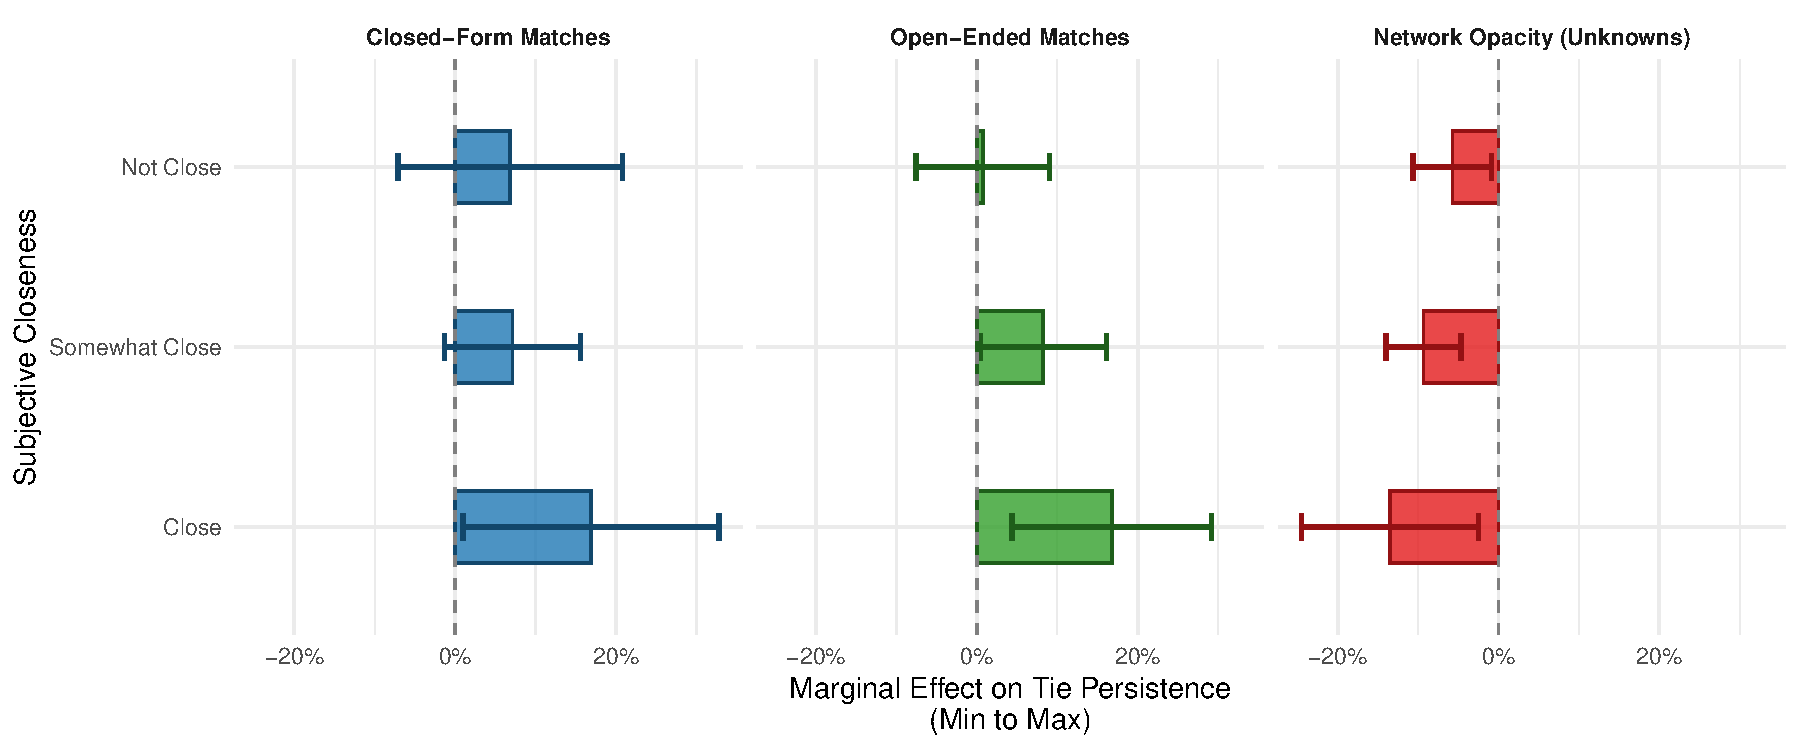
\includegraphics[keepaspectratio]{analysis_files/figure-pdf/fig-closeness-interactions-1.pdf}}

}

\caption{\label{fig-closeness-interactions}Marginal Effects of Cultural
Matching and Network Opacity by Subjective Closeness}

\end{figure}%

As the marginal effects plot demonstrates, the moderating role of
subjective closeness varies by the type of cultural measure. For
closed-form matches and network opacity, there is a strong interaction
with tie strength: the marginal effects are steepest for ``Not Close''
ties, indicating that broad cultural alignment and mutual cultural
knowledge provide critical scaffolding that helps weak ties survive.
Conversely, for ties that are already ``Close,'' the slopes for
closed-form matches and opacity are much flatter, suggesting these
strong ties are more resilient to decay regardless of these factors. In
contrast, open-ended matches do not show as strong of an interaction;
their protective effect remains relatively consistent across different
levels of subjective closeness. \newpage

\subsection{Appendix: Descriptive
Statistics}\label{appendix-descriptive-statistics}

\subsection{Robustness Check: Ego Fixed
Effects}\label{robustness-check-ego-fixed-effects}

To ensure the robustness of our main findings, we estimated an
\textbf{Ego Fixed-Effects} model using conditional logistic regression
(\texttt{survival::clogit}). This stringent test completely controls for
all unobserved, time-invariant ego characteristics by only leveraging
within-ego variance (i.e., comparing alters retained vs.~dropped by the
same ego).




\end{document}
